%
%       Git documentation.tex
%
%       Copyright 2011 Miguel Sánchez de León Peque <msdeleonpeque at gmail dot com>
%
%       This program is free software; you can redistribute it and/or modify
%       it under the terms of the GNU General Public License as published by
%       the Free Software Foundation; either version 3 of the License, or
%       (at your option) any later version.
%
%       This program is distributed in the hope that it will be useful,
%       but WITHOUT ANY WARRANTY; without even the implied warranty of
%       MERCHANTABILITY or FITNESS FOR A PARTICULAR PURPOSE.  See the
%       GNU General Public License for more details.
%
%       You should have received a copy of the GNU General Public License
%       along with this program; if not, write to the Free Software
%       Foundation, Inc., 51 Franklin Street, Fifth Floor, Boston,
%       MA 02110-1301, USA.
%


\documentclass[a4paper,10pt]{article}

\usepackage[english]{babel}
\usepackage{graphicx}
\usepackage{listings}
\usepackage{geometry}
\usepackage{framed}
\usepackage{multirow}
\usepackage{peque}

\newcommand{\projectname}{cookie-libs}
\newcommand{\projectgitrepo}{git://cookie-libs.git.sourceforge.net/gitroot/cookie-libs/cookie-libs}
\newcommand{\projectsshgitrepo}{ssh://USERNAME@cookie-libs.git.sourceforge.net/gitroot/cookie-libs/cookie-libs}

% TODO: Implicit verbatim environment in terminal environment.
\newenvironment{terminal}
  {
    \vspace{+10pt}
    \begin{center}
    \begin{minipage}{0.95\textwidth}
    \begin{framed}
  }
  {
    \end{framed}
    \end{minipage}
    \end{center}
    \vspace{+10pt}
  }


\begin{document}

\begin{titlepage}
\begin{center}
	\ \\%
	\vspace{8.0cm}
	\LARGE{\textbf{Git documentation}} \\
	\vspace{1.0cm}
	\Large{Miguel Sánchez de León Peque} \\
	\vspace{0.5cm}
	\large{\today}
\end{center}
\end{titlepage}
\thispagestyle{empty}
\cleardoublepage


\pagenumbering{roman}

\tableofcontents
\cleardoublepage


\listoffigures
\listoftables
\cleardoublepage


\pagenumbering{arabic}


\section{Introduction}

\subsection{Collaborative projects}

When software is developed by a group of programmers, some method is
necessary to control access and track changes made in source code.

Version control (also known as revision or source control) is the art of
managing software through its process of development.

Every change is usually identified by a number or letter code which is
called the revision number (or simply revision). Each revision is
associated with a time stamp and the person making the change.

\subsection{Distributed version control systems}

A distributed version control system allows developers to work on a
project without needing to be connected to a common network.

In centralized systems (such as the well known Subversion) there is a
client-server approach, while in distributed systems there is a
peer-to-peer approach. That means there are only working and full
functional copies: common operations (such as commits, viewing history,
and reverting changes) are fast, because there is no need to communicate
with a central server. Furthermore, this provides natural protection
against data loss. Communication is only necessary when pulling or
pushing changes from or to other peers.

\section{Git}

\subsection{About Git}

Git is a distributed version control system which was initially designed
by Linus Torvalds\footnote{Linus Torvalds started the Linux project back
in 1991. The Linux kernel has become the \textit{de facto} standard
kernel for almost all GNU distributions.} for the Linux kernel
development. Just as the Linux kernel, Git has been released as free
software\footnote{The term \textit{free} refers to software that can be
used, studied, and modified without restriction, and which can be copied
and redistributed in modified or unmodified form (\textit{free} as in
\textit{freedom}).} under the General Public License (GPL).

It is probably the best version control system ever made as it has probed
to be amazingly fast (specially on POSIX-based systems) and versatile.
It is the most used in new software projects and many older projects have
started using it. Some important projects that are currently using Git
are:
Linux kernel,
GIMP,
Git (itself),
VLC media player,
Android,
Eclipse,
jQuery,
PostgreSQL,
Wine,
Chromium (Google Chrome),
Perl,
KDE,
GNOME,
Qt 4,
GTK+,
phpBB,
many GNU projects (GNU Compiler Collection, GNU C library, grep, tar...),
Drupal,
X.Org,
rsync,
and many, many more.

\subsection{Git overview}

Most projects have a main or master branch where stable code is kept. Changes
which will quickly add new functionality or fix bugs are made here (figure
\ref{master-branch}).

\begin{figure}
  \begin{center}
    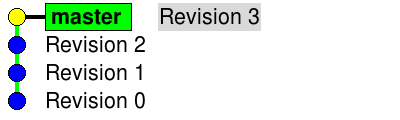
\includegraphics[scale=0.5]{branching-00}
  \end{center}
  \caption{Development in master branch}
  \label{master-branch}
\end{figure}

Whenever you want to start developing a bigger new feature or code refactoring,
you should better not be in the master branch, as the first changes will
probably introduce some errors to the master branch, where others may be coding
at that time. If you break the project's functionality in the main branch, you
will stop other developers from doing their job.

The best thing you can do is to create a new branch (figure
\ref{create-new-branch}). That way, you will have all the advantages of the
version control system, but your changes wont affect , at least for now, other
developers. You may want to share this branch with other developers (uploading
it to the server) or keep it locally until the job is done.

\begin{figure}
  \begin{center}
    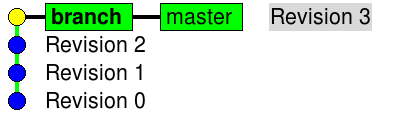
\includegraphics[scale=0.5]{branching-01}
  \end{center}
  \caption{Creating a new branch}
  \label{create-new-branch}
\end{figure}

Once you are in the new branch, you can start making changes just as in
the master branch (figure \ref{development-in-your-own-branch}).

\begin{figure}
  \begin{center}
    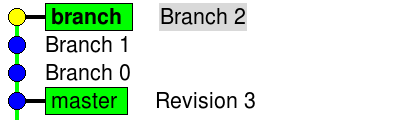
\includegraphics[scale=0.5]{branching-02}
  \end{center}
  \caption{Development in your own branch}
  \label{development-in-your-own-branch}
\end{figure}

Notice that while you are working on your branch, development may occur
simultaneously in the master branch, or in any other branch (figure
\ref{simultaneous-development}). But do not worry, because those changes wont
affect your branch either.

\begin{figure}
  \begin{center}
    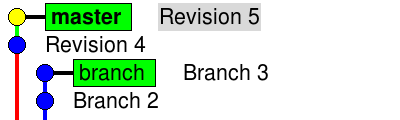
\includegraphics[scale=0.5]{branching-03}
  \end{center}
  \caption{Simultaneous development}
  \label{simultaneous-development}
\end{figure}

Once you are done with your branch, you will only need to merge those
changes with the master branch (figure \ref{merging-changes}).

\begin{figure}
  \begin{center}
    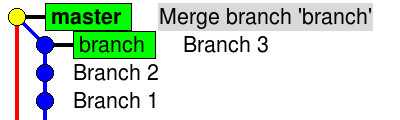
\includegraphics[scale=0.5]{branching-04}
  \end{center}
  \caption{Merging changes}
  \label{merging-changes}
\end{figure}

\subsection{Git interface}

Although there might be some GUIs for Git, we will be using the command-line
interface which, once you get used to it, will bring you the way to reach the
best results.

Every command you will use will start with the word \texttt{git}, followed
by the task you want to perform. Some examples are:
\texttt{git status},
\texttt{git add <filename>},
\texttt{git commit -m 'Changes you made'}...

We will be learning more about this commands soon, but first, why do not we
check out an example?

\section{A Git example}

\subsection{First steps on Git}

Installing Git is really simple in GNU/Linux systems. You can use your
package manager or, alternatively, the terminal. For example, in
Fedora, installing Git would be as easy as:

\begin{terminal}
\begin{verbatim}
$ sudo dnf install -y git gitk
\end{verbatim}
\end{terminal}

To initialize a Git repository, create an empty folder which will
contain the full project.

\begin{terminal}
\begin{verbatim}
$ mkdir git-test
$ cd git-test
$ git init
\end{verbatim}
\end{terminal}

The command \texttt{git init} initializes an empty Git repository in
\texttt{git-test} folder. That will allow you to perform many other Git
operations in the future, when some changes are made within the project.

Now, let us create a file named \texttt{test-file.txt}, with one text
line:

\begin{terminal}
\begin{verbatim}
$ echo Line 0 > test-file.txt
\end{verbatim}
\end{terminal}

That would be our initial commit.

\begin{terminal}
\begin{verbatim}
$ git add .
$ git commit -m 'Initial commit'
\end{verbatim}
\end{terminal}

We will use the \texttt{git add} command whenever we want to confirm
changes for a commit. In this case, we are adding the whole current
folder '\texttt{.}', which is \texttt{git-test}. After adding the
changes we made, we will make the commit to create the next revision.
A commit is essentially giving a description to the changes we added.
The option \texttt{-m} will let us easily add a short description to
the commit. The description must be written after the \texttt{-m} option
and between simple quotes.

\begin{tip}
You may ommit the \texttt{-m} option but, doing so, you will enter a
console editor (such as Vi) for writting your description. Managing this
editors is not the matter of this documentation.
\end{tip}

There is a command we can use to see the project status. It will show
us the branch we are working in, the files or folders we changed
(added, deleted or modified), which of them are already added and if
there are still commits waiting to be uploaded to the server. In our
example, we can see we are in the \texttt{master} branch, and we have
no changes to be commited.

\begin{terminal}
\begin{verbatim}
$ git status
# On branch master
nothing to commit (working directory clean)
\end{verbatim}
\end{terminal}

Let us say we make a change to the \texttt{text-file.txt}. Let us delete the
line we wrote and write a new one.

\begin{terminal}
\begin{verbatim}
$ echo New line 0 > test-file.txt
\end{verbatim}
\end{terminal}

Now, our status has changed:

\begin{terminal}
\begin{verbatim}
$ git status
# On branch master
# Changes not staged for commit:
#   (use "git add <file>..." to update what will be committed)
#   (use "git checkout -- <file>..." to discard changes in working dir.)
#
#	modified:   test-file.txt
#
no changes added to commit (use "git add" and/or "git commit -a")
\end{verbatim}
\end{terminal}

We can see \texttt{text-file.txt} has been modified. As Git is
suggesting, we have got two options to perform: add the changes for a
later commit (\texttt{git add text-file.txt}) or discard those changes
(\texttt{git checkout -{}- text-file.txt}). But before continuing, let us
introduce a new tool: \texttt{gitk}.

\texttt{gitk} is a graphical interface that will allow us to easily
checkout the project's history and also the local changes we make. Let us
see how it looks like.

\begin{terminal}
\begin{verbatim}
$ gitk
\end{verbatim}
\end{terminal}

On the upper-left of the window, we can see the history tree, where
each commit is represented by a circle and its description. In our
example, this consist only in the initial commit and a red circle which
represents some changes that have not been added yet.

\begin{figure}
  \begin{center}
    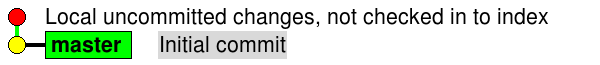
\includegraphics[scale=0.5]{git_example-00}
  \end{center}
  \caption{Unstaged changes}
\end{figure}

At the right of each revision or commit, we can see the name of the
committer with his or her email and the date the commit was made.

\begin{tip}
Notice that you have not configured your name and email address, so,
although you made the initial commit, your name and email wont be
displayed (instead, you will find some session and system information).
\end{tip}

We can navigate through the history tree to see the changes that were
made in each of them. If we select the upper line (local uncommitted
changes), we will see the following information:

\begin{figure}
  \begin{center}
    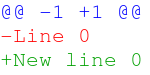
\includegraphics[scale=0.5]{git_example-01}
  \end{center}
  \caption{Diff file}
\end{figure}

Red lines represent those which have been deleted, and green lines those
which have been added. On the right, we can see a list of the files
that have been modified.

So, lest now close the window and go back to the terminal. We want to
confirm the changes we made, as we have already reviewed them with the
\texttt{gitk} tool. So, we need to add them:

\begin{terminal}
\begin{verbatim}
$ git add test-file.txt
\end{verbatim}
\end{terminal}

Let us see what happened.

\begin{terminal}
\begin{verbatim}
$ git status
# On branch master
# Changes to be committed:
#   (use "git reset HEAD <file>..." to unstage)
#
#	modified:   test-file.txt
#
\end{verbatim}
\end{terminal}

And if we use the \texttt{gitk} tool, we will see the upper line has now
a green circle, which represents changes waiting to be commited.

\begin{figure}
  \begin{center}
    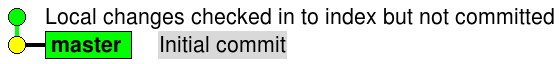
\includegraphics[scale=0.5]{git_example-02}
  \end{center}
  \caption{Changes to be commited}
\end{figure}

Now we can do two things: make the commit (\texttt{git commit -m
'Changed line in test-file.txt'}) or revert the last operation
(\texttt{git reset HEAD test-file.txt}) to unstage the file. If the
perform the last operation, we will see again a red circle with
\texttt{gitk}, which means changes need to be added again. But normally,
we want to commit the changes:

\begin{terminal}
\begin{verbatim}
$ git commit -m 'Changed line in test-file.txt'
[master 107f4e6] Changed line in test-file.txt
 1 files changed, 1 insertions(+), 1 deletions(-)
$ git status
# On branch master
nothing to commit (working directory clean)
\end{verbatim}
\end{terminal}

The \texttt{gitk} tool will show us a new commit:

\begin{figure}
  \begin{center}
    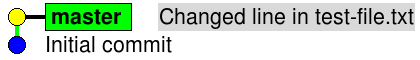
\includegraphics[scale=0.5]{git_example-03}
  \end{center}
  \caption{New revision in the history tree}
\end{figure}

Normally, we will keep working and making new commit, but there is a
chance that (even if we "checked" it before with \texttt{gitk}) we
made an erroneous commit. Again, we have got two options: we can make
a new commit to correct the last one or, if you did not already pushed
your changes to the server (which is something we have not talked about
yet), undo the last commit in the local tree:

\begin{terminal}
\begin{verbatim}
$ git reset --soft HEAD^
\end{verbatim}
\end{terminal}

That way, we will go back to the previous status.

\begin{tip}
Using the \texttt{-{}-soft} option is highly recommended, as other
options (as \texttt{-{}-hard}) will also unstage the changes. Try to
always perform this operations step by step. Remember: it is for your
own safety!
\end{tip}

\subsection{Branching}

Now that we know how to make commits, let us get into branching. You can
easily change between branches using
\texttt{git checkout <branch\_name>}
but, you will need to add the \texttt{-b} option if the branch does not
exist (that way, you will create a new branch called
\texttt{<branch\_name>}).

\begin{terminal}
\begin{verbatim}
$ git checkout -b newbr
Switched to a new branch 'newbr'
\end{verbatim}
\end{terminal}

Now we are exactly at the same revision as before, but in a new branch.

\begin{figure}
  \begin{center}
    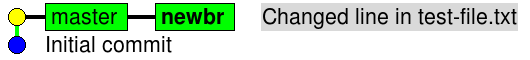
\includegraphics[scale=0.5]{git_example-04}
  \end{center}
  \caption{New branch}
\end{figure}

\begin{tip}
Important: \texttt{gitk} shows by default the history of the branch we
are currently in. If we want to see the full tree, we need to use the
\texttt{-{}-all} option: \texttt{gitk -{}-all}. For now on, we will be
using that option whenever we need to use the \texttt{gitk} tool.
\end{tip}

So, let us add a new line to our \texttt{test-file.txt} and commit the
changes:

\begin{terminal}
\begin{verbatim}
$ echo Line 1 written from newbr branch >> test-file.txt
$ git add test-file.txt
$ git commit -m 'Added line 1 to test-file.txt'
[newbr 405f629] Added line 1 to test-file.txt
 1 files changed, 1 insertions(+), 0 deletions(-)
\end{verbatim}
\end{terminal}


Now, our branch \texttt{newbr} is ahead in the history tree as the
commit we made has not affect the \texttt{master} branch.

\begin{figure}
  \begin{center}
    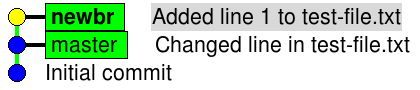
\includegraphics[scale=0.5]{git_example-05}
  \end{center}
  \caption{New commit in \texttt{newbr} branch}
\end{figure}

But, what happens if a new commit is made in the \texttt{master}
branch? Let us change to it and make a new commit from there:

\begin{terminal}
\begin{verbatim}
$ git checkout master
Switched to branch 'master'
$ echo Line 1 written from master branch >> test-file.txt
$ git add test-file.txt
$ git commit -m 'Added line 1 to test-file.txt'
[master c373bbc] Added line 1 to test-file.txt
 1 files changed, 1 insertions(+), 0 deletions(-)
\end{verbatim}
\end{terminal}

\begin{tip}
Notice that when we change from one branch to another, all the files
within the project's folder change to the situation in which they are
in the new branch.
\end{tip}

Now the \texttt{master} branch is ahead in the history tree.

\begin{figure}
  \begin{center}
    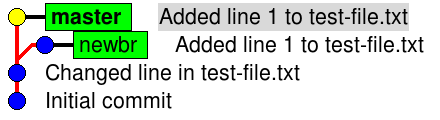
\includegraphics[scale=0.5]{git_example-06}
  \end{center}
  \caption{New commit in \texttt{master} branch}
\end{figure}

Let us say we finished making changes in \texttt{newbr} branch. Now, we
would like to merge the changes we made with the master branch (we
need to do that from the branch we want to merge the changes to: in
this case from \texttt{master}).

\begin{terminal}
\begin{verbatim}
$ git merge newbr
Auto-merging test-file.txt
CONFLICT (content): Merge conflict in test-file.txt
Automatic merge failed; fix conflicts and then commit the result.
\end{verbatim}
\end{terminal}

What happened here? Well, sometimes when you are working in a project
with other people, you may find that others have made changes to the
same sources you are working on in your branch. In our example, the
second line of the file was modified in both branches, and Git does not
know which one should it take.

Let us see what Git says about this status:

\begin{terminal}
\begin{verbatim}
$ git status
# On branch master
# Unmerged paths:
#   (use "git add/rm <file>..." as appropriate to mark resolution)
#
#	both modified:      test-file.txt
#
no changes added to commit (use "git add" and/or "git commit -a")
\end{verbatim}
\end{terminal}

For solving merging conflicts manually, we will first a look at the
history tree with \texttt{gitk}. We will find which lines conflict in
the file.

\begin{figure}
  \begin{center}
    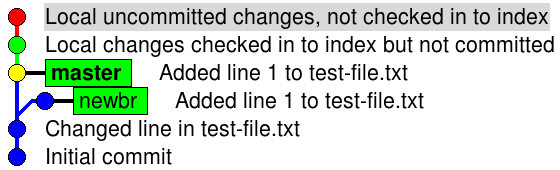
\includegraphics[scale=0.5]{git_example-07}
  \end{center}
  \caption{History tree after a merging conflict}
\end{figure}

\begin{figure}
  \begin{center}
    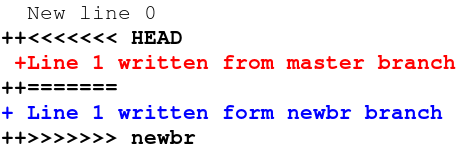
\includegraphics[scale=0.5]{git_example-08}
  \end{center}
  \caption{Conflicting lines}
\end{figure}

Those lines in red color, which are under the \texttt{HEAD} tag,
represent changes in our current branch (\texttt{master}). Those in
blue, which are over the \texttt{newbr} tag, represent changes in the
\texttt{newbr} branch. What we need to do is to open the file and
remove those lines we do not want to keep there.

Let us say we want to keep the changes we made in the \texttt{newbr}
branch. We need to delete the line in red (which corresponds to the
line added from the \texttt{master} branch) and also the delimiter
lines that Git added to the file to separate the conflicting lines.

If we do that correctly, we can complete the merge just as if we were
making a normal commit:

\begin{terminal}
\begin{verbatim}
$ git add test-file.txt
$ git commit -m 'Merge branch newbr into master (conflicts solved)'
[master aea5947] Merge branch newbr into master (conflicts solved)
\end{verbatim}
\end{terminal}

\begin{figure}
  \begin{center}
    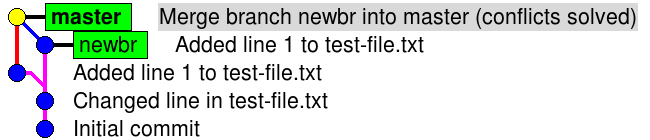
\includegraphics[scale=0.5]{git_example-09}
  \end{center}
  \caption{Branch \texttt{newbr} merged into \texttt{master}}
\end{figure}

\begin{tip}
Conflicts while merging branches may happen to you from time to time,
specially if you modified many files or if many other
people are working at the same time in the project. Git usually solves
most of the conflicts by it self though.
\end{tip}

\section{Working with Git in the \projectname\ project}

\subsection{Cloning an already existing repository}

The \projectname\ project is already hosted in a server, more precisely
in SourceForge. That means you will need to have a SourceForge account
and you will need to ask the administrator to join the developers team
in order to have write permissions in the server.

\begin{tip}
You can contribute to the \projectname\ project without being part of
the developers team, generating and sending patches to them. Anyway,
we will not cover how to make patches within this document.
\end{tip}

Once you have joined the development team, you can clone the server's
repository to create a local copy of the project to work with. The
\texttt{USERNAME} is your SourceForge user's name and the
password you are asked for is your SourceForge's as well:

\begin{terminal}
\begin{verbatim}
$ git clone ssh://USERNAME@cookie-libs.git.sourceforge.net/gitroot/\
cookie-libs/cookie-libs

Cloning into cookie-libs...
USERNAME@cookie-libs.git.sourceforge.net's password:
remote: Counting objects: 452, done.
remote: Compressing objects: 100% (447/447), done.
remote: Total 452 (delta 251), reused 0 (delta 0)
Receiving objects: 100% (452/452), 5.24 MiB | 109 KiB/s, done.
Resolving deltas: 100% (251/251), done.
\end{verbatim}
\end{terminal}

Once the process has been completed, you will see a folder called
\texttt{cookie-libs} in which you will find the entire project. Inside
the folder, you will be able to use the Git command line interface and
the \texttt{gitk} tool as you did before, as it is a local repository
as well.

\begin{terminal}
\begin{verbatim}
$ cd cookie-libs
$ git status
# On branch master
nothing to commit (working directory clean)
\end{verbatim}
\end{terminal}

Before starting making changes, as we will be now sharing our work with
the rest of the developers, we will need to configure Git so that it will
associate our commits with our name and email address\footnote{Using
our real name and email address is important for other developers to
know who are you and how to contact you in case they need it.}.

\begin{terminal}
\begin{verbatim}
$ git config --global user.name "Here Comes My Name"
$ git config --global user.email "here.comes@my.email"
\end{verbatim}
\end{terminal}

Do not forget the \texttt{" "} around your name and email! If you want
to check your configuration, just execute:

\begin{terminal}
\begin{verbatim}
$ git config -l
\end{verbatim}
\end{terminal}

You should see your name and email address displayed (among other
things).

\subsection{Git, from local to server}

Although everything is very similar, you may notice one difference:
there are two tags in the latest
revision. Those tags correspond to the local branch (\texttt{master})
and the remote
branch (\texttt{remotes/origin/master}).

\begin{figure}
  \begin{center}
    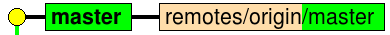
\includegraphics[scale=0.5]{server-00}
  \end{center}
  \caption{Both the local and remote \texttt{master} branches}
\end{figure}

You can work in your local copy with the same commands we have
learned, but, once you make a commit, it will be written only in your
local \texttt{master} branch.

\begin{figure}
  \begin{center}
    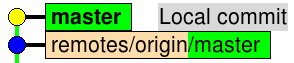
\includegraphics[scale=0.5]{server-01}
  \end{center}
  \caption{New local commit}
\end{figure}

Of course, we can keep doing local development but, at some time, we
will want to share our changes with the other developers, so we will
upload them to the server (also it is safer to have a copy of your
local work). To do so, we will use the \texttt{push} command once we have
already made the commit in our local repository.

\begin{terminal}
\begin{verbatim}
$ git push
\end{verbatim}
\end{terminal}

\begin{figure}
  \begin{center}
    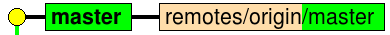
\includegraphics[scale=0.5]{server-00}
  \end{center}
  \caption{Again, both local and remote branches are at the same revision}
\end{figure}

Although it is possible, we encorage you not to undo commits that you
have already pushed to the server. If you want to fix your last
commit, just create a new one with the necessary changes. If you want
to undo the last commit, you can revert the changes you made:

\begin{terminal}
\begin{verbatim}
$ git revert <SHA1 ID>
\end{verbatim}
\end{terminal}

Where \texttt{<SHA1 ID>} is the commit's ID (or the begining of
it)\footnote{You can execute \texttt{git revert
0e81e5588b4da07a4ff8388fee01dfed776a7e14} or \texttt{git revert 0e81e}}.

Just as simple! There is only one more thing: how can we download
changes from the server? (those which other developers made). That is
a very simple task too:

\begin{terminal}
\begin{verbatim}
$ git pull
\end{verbatim}
\end{terminal}

\begin{tip}
Remember to use \texttt{git pull} frequently, so you can have your
local copy updated and notice what other developers are doing within
the project.
\end{tip}

\subsection{Remote branches}

Working with remote branches has the same problem. Local changes do not
apply until we execute the corresponding command. Once we have created
a local branch, we can initialize it in the server with:

\begin{terminal}
\begin{verbatim}
$ git push origin new_branch_name
\end{verbatim}
\end{terminal}

Once the branch has been initialized, we can share our changes with a
normal \texttt{git push}.

If we want to download changes in a specific branch, we can use:

\begin{terminal}
\begin{verbatim}
$ git pull origin branch_name
\end{verbatim}
\end{terminal}

Again, it is not a good idea to delete branches from the server once
we have pushed them. Anyway, if we already finished working with one
branch and it has been already merged with the \texttt{master} branch,
we may want to delete it to keep the history tree clean. First, we will
delete our local branch:

\begin{terminal}
\begin{verbatim}
$ git branch -d branch_name
\end{verbatim}
\end{terminal}

\begin{tip}
If we started a branch that we do not want to merge with the
\texttt{master} branch (we may have started developing a crazy idea)
and we want to delete it either way, we can use the command
\texttt{git branch -D branch\_name}.
\end{tip}

After that, and after consulting other developers in the project, we
can delete the remote branch:

\begin{terminal}
\begin{verbatim}
$ git push origin :branch_name
\end{verbatim}
\end{terminal}

\section{Git command reference}

\subsection{Commands we have reviewed withing this document}

\begin{table}
\caption{Initial configuration}
\centering
\begin{tabular}{l l l}
\hline\hline
Command & Options & Description \\
\hline\hline
\multirow{1}{*}{\texttt{clone}} & \texttt{<git\_repo>} & Clone a remote Git repository \\ \hline
\multirow{3}{*}{\texttt{config}} & \texttt{-{}-global user.name <user\_name>} & Configure user's name \\
& \texttt{-{}-global user.email <user\_email>} & Configure user's mail \\
& \texttt{-l} & List configuration settings \\ \hline
\hline
\end{tabular}
\end{table}

\begin{table}
\caption{Simple commands}
\centering
\begin{tabular}{l l l}
\hline\hline
Command & Options & Description \\
\hline\hline
\multirow{1}{*}{\texttt{status}} & (none) & Show current status \\ \hline
\multirow{1}{*}{\texttt{add}} & \texttt{<file\_name>} & Confirm changes to be commited (new files) \\ \hline
\multirow{1}{*}{\texttt{rm}} & \texttt{<file\_name>} & Confirm changes to be commited (deleted files) \\ \hline
\multirow{3}{*}{\texttt{commit}} & (none) & Edit commit's description with a command line editor \\
& \texttt{-a} & Commit all changes (even those not confirmed yet) \\
& \texttt{-m} & Commit's description \\ \hline
\multirow{1}{*}{\texttt{revert}} & \texttt{<commit\_ID>} & Revert one commit \\ \hline
\multirow{3}{*}{\texttt{reset}} & \texttt{-{}-soft HEAD\^} & Undo last local commit  \\
& \texttt{-{}-hard HEAD\^} & Undo all the changes in last local commit \\
& \texttt{HEAD <file\_name>} & Unconfirm added changes \\ \hline
\multirow{1}{*}{\texttt{pull}} & (none) & Download remote changes from the server  \\ \hline
\multirow{1}{*}{\texttt{push}} & (none) & Upload local commits to the server  \\ \hline
\hline
\end{tabular}
\end{table}

\begin{table}
\caption{Working with branches}
\centering
\begin{tabular}{l l l}
\hline\hline
Command & Options & Description \\
\hline\hline
\multirow{2}{*}{\texttt{push}} & \texttt{origin <new\_branch\_mame>} & Initialize new local branch in the server \\
& \texttt{origin :<branch\_name>} & Delete remote branch (use with care!) \\ \hline
\multirow{1}{*}{\texttt{pull}} & \texttt{origin <branch\_name>} & Download changes from the remote branch  \\ \hline
\multirow{1}{*}{\texttt{merge}} & \texttt{<branch\_name>} & Merge \texttt{<branch\_name>} to the current branch \\ \hline
\multirow{2}{*}{\texttt{checkout}} & \texttt{<branch\_name>} & Move to \texttt{<branch\_name>}  \\
& \texttt{-b <new\_branch\_name>} & Create a new branch \texttt{<branch\_name>} \\ \hline
\multirow{2}{*}{\texttt{branch}} & \texttt{-d <branch\_name>} & Delete \texttt{<branch\_name>} (once merged) \\
& \texttt{-D <branch\_name>} & Delete branch irrespective of its merged status \\ \hline
\hline
\end{tabular}
\end{table}

\subsection{More useful commands}

\begin{table}
\caption{Working with tags}
\centering
\begin{tabular}{l l l}
\hline\hline
Command & Options & Description \\
\hline\hline
\multirow{3}{*}{\texttt{tag}} & (none) & List all tags \\
 & \texttt{-a <tag\_name>} & Add the tag name \\
 & \texttt{-m '<tag\_desc>'} & Add the tag description \\ \hline
\multirow{2}{*}{\texttt{push origin}} & \texttt{-{}-tags} & Push all tags to the server \\
 & \texttt{<tag\_name>} & Push tag (with <tag\_name>) to the server \\ \hline
\hline
\end{tabular}
\end{table}

Example:

\begin{terminal}
\begin{verbatim}
$ git tag -a v0.1 -m 'versión 0.1'
$ git push origin v0.1
\end{verbatim}
\end{terminal}

\begin{table}
\caption{Patching}
\centering
\begin{tabular}{l l l}
\hline\hline
Command & Options & Description \\
\hline\hline
\multirow{1}{*}{\texttt{format-patch}} & \texttt{origin/branch\_name} & Create a patch for remote \texttt{branch\_name} \\ \hline
\multirow{1}{*}{\texttt{apply}} & \texttt{<patch\_name>} & Apply patch in the project \\ \hline
\end{tabular}
\end{table}

Example:

\begin{terminal}
\begin{verbatim}
$ git format-patch origin/master
$ git apply filename.patch
\end{verbatim}
\end{terminal}

\end{document}
